% Options for packages loaded elsewhere
\PassOptionsToPackage{unicode}{hyperref}
\PassOptionsToPackage{hyphens}{url}
%
\documentclass[
]{article}
\usepackage{amsmath,amssymb}
\usepackage{lmodern}
\usepackage{ifxetex,ifluatex}
\ifnum 0\ifxetex 1\fi\ifluatex 1\fi=0 % if pdftex
  \usepackage[T1]{fontenc}
  \usepackage[utf8]{inputenc}
  \usepackage{textcomp} % provide euro and other symbols
\else % if luatex or xetex
  \usepackage{unicode-math}
  \defaultfontfeatures{Scale=MatchLowercase}
  \defaultfontfeatures[\rmfamily]{Ligatures=TeX,Scale=1}
\fi
% Use upquote if available, for straight quotes in verbatim environments
\IfFileExists{upquote.sty}{\usepackage{upquote}}{}
\IfFileExists{microtype.sty}{% use microtype if available
  \usepackage[]{microtype}
  \UseMicrotypeSet[protrusion]{basicmath} % disable protrusion for tt fonts
}{}
\makeatletter
\@ifundefined{KOMAClassName}{% if non-KOMA class
  \IfFileExists{parskip.sty}{%
    \usepackage{parskip}
  }{% else
    \setlength{\parindent}{0pt}
    \setlength{\parskip}{6pt plus 2pt minus 1pt}}
}{% if KOMA class
  \KOMAoptions{parskip=half}}
\makeatother
\usepackage{xcolor}
\IfFileExists{xurl.sty}{\usepackage{xurl}}{} % add URL line breaks if available
\IfFileExists{bookmark.sty}{\usepackage{bookmark}}{\usepackage{hyperref}}
\hypersetup{
  pdftitle={DAP Project},
  pdfauthor={Daniel Granja},
  hidelinks,
  pdfcreator={LaTeX via pandoc}}
\urlstyle{same} % disable monospaced font for URLs
\usepackage[margin=1in]{geometry}
\usepackage{color}
\usepackage{fancyvrb}
\newcommand{\VerbBar}{|}
\newcommand{\VERB}{\Verb[commandchars=\\\{\}]}
\DefineVerbatimEnvironment{Highlighting}{Verbatim}{commandchars=\\\{\}}
% Add ',fontsize=\small' for more characters per line
\usepackage{framed}
\definecolor{shadecolor}{RGB}{248,248,248}
\newenvironment{Shaded}{\begin{snugshade}}{\end{snugshade}}
\newcommand{\AlertTok}[1]{\textcolor[rgb]{0.94,0.16,0.16}{#1}}
\newcommand{\AnnotationTok}[1]{\textcolor[rgb]{0.56,0.35,0.01}{\textbf{\textit{#1}}}}
\newcommand{\AttributeTok}[1]{\textcolor[rgb]{0.77,0.63,0.00}{#1}}
\newcommand{\BaseNTok}[1]{\textcolor[rgb]{0.00,0.00,0.81}{#1}}
\newcommand{\BuiltInTok}[1]{#1}
\newcommand{\CharTok}[1]{\textcolor[rgb]{0.31,0.60,0.02}{#1}}
\newcommand{\CommentTok}[1]{\textcolor[rgb]{0.56,0.35,0.01}{\textit{#1}}}
\newcommand{\CommentVarTok}[1]{\textcolor[rgb]{0.56,0.35,0.01}{\textbf{\textit{#1}}}}
\newcommand{\ConstantTok}[1]{\textcolor[rgb]{0.00,0.00,0.00}{#1}}
\newcommand{\ControlFlowTok}[1]{\textcolor[rgb]{0.13,0.29,0.53}{\textbf{#1}}}
\newcommand{\DataTypeTok}[1]{\textcolor[rgb]{0.13,0.29,0.53}{#1}}
\newcommand{\DecValTok}[1]{\textcolor[rgb]{0.00,0.00,0.81}{#1}}
\newcommand{\DocumentationTok}[1]{\textcolor[rgb]{0.56,0.35,0.01}{\textbf{\textit{#1}}}}
\newcommand{\ErrorTok}[1]{\textcolor[rgb]{0.64,0.00,0.00}{\textbf{#1}}}
\newcommand{\ExtensionTok}[1]{#1}
\newcommand{\FloatTok}[1]{\textcolor[rgb]{0.00,0.00,0.81}{#1}}
\newcommand{\FunctionTok}[1]{\textcolor[rgb]{0.00,0.00,0.00}{#1}}
\newcommand{\ImportTok}[1]{#1}
\newcommand{\InformationTok}[1]{\textcolor[rgb]{0.56,0.35,0.01}{\textbf{\textit{#1}}}}
\newcommand{\KeywordTok}[1]{\textcolor[rgb]{0.13,0.29,0.53}{\textbf{#1}}}
\newcommand{\NormalTok}[1]{#1}
\newcommand{\OperatorTok}[1]{\textcolor[rgb]{0.81,0.36,0.00}{\textbf{#1}}}
\newcommand{\OtherTok}[1]{\textcolor[rgb]{0.56,0.35,0.01}{#1}}
\newcommand{\PreprocessorTok}[1]{\textcolor[rgb]{0.56,0.35,0.01}{\textit{#1}}}
\newcommand{\RegionMarkerTok}[1]{#1}
\newcommand{\SpecialCharTok}[1]{\textcolor[rgb]{0.00,0.00,0.00}{#1}}
\newcommand{\SpecialStringTok}[1]{\textcolor[rgb]{0.31,0.60,0.02}{#1}}
\newcommand{\StringTok}[1]{\textcolor[rgb]{0.31,0.60,0.02}{#1}}
\newcommand{\VariableTok}[1]{\textcolor[rgb]{0.00,0.00,0.00}{#1}}
\newcommand{\VerbatimStringTok}[1]{\textcolor[rgb]{0.31,0.60,0.02}{#1}}
\newcommand{\WarningTok}[1]{\textcolor[rgb]{0.56,0.35,0.01}{\textbf{\textit{#1}}}}
\usepackage{graphicx}
\makeatletter
\def\maxwidth{\ifdim\Gin@nat@width>\linewidth\linewidth\else\Gin@nat@width\fi}
\def\maxheight{\ifdim\Gin@nat@height>\textheight\textheight\else\Gin@nat@height\fi}
\makeatother
% Scale images if necessary, so that they will not overflow the page
% margins by default, and it is still possible to overwrite the defaults
% using explicit options in \includegraphics[width, height, ...]{}
\setkeys{Gin}{width=\maxwidth,height=\maxheight,keepaspectratio}
% Set default figure placement to htbp
\makeatletter
\def\fps@figure{htbp}
\makeatother
\setlength{\emergencystretch}{3em} % prevent overfull lines
\providecommand{\tightlist}{%
  \setlength{\itemsep}{0pt}\setlength{\parskip}{0pt}}
\setcounter{secnumdepth}{-\maxdimen} % remove section numbering
\usepackage{booktabs}
\usepackage{longtable}
\usepackage{array}
\usepackage{multirow}
\usepackage{wrapfig}
\usepackage{float}
\usepackage{colortbl}
\usepackage{pdflscape}
\usepackage{tabu}
\usepackage{threeparttable}
\usepackage{threeparttablex}
\usepackage[normalem]{ulem}
\usepackage{makecell}
\usepackage{xcolor}
\ifluatex
  \usepackage{selnolig}  % disable illegal ligatures
\fi

\title{DAP Project}
\author{Daniel Granja}
\date{10/12/2021}

\begin{document}
\maketitle

\hypertarget{introduction}{%
\section{Introduction}\label{introduction}}

\hypertarget{context-of-the-project}{%
\subsection{Context of the project}\label{context-of-the-project}}

According to the American Psychological Association (APA), emotion is
defined as ``a complex reaction pattern, involving experiential,
behavioral and physiological elements.'' Researchers have been studying
the impact of emotions on cognitive functions, such as memory. Studies
have shown that emotional activation, and specifically emotions of
negative valence, favours the retrieval processes of associative memory
for single items, but impairs it for associated items or contexts
(Schmidt, Patnaik \& Kensinger, 2010). It's believed that the
neurobiological systems sustaining high emotional arousal and memory are
linked, especially through the adrenal stress hormones, itself mediated
by the amygdala activity (McGaugh, 2013). In the study the dataset came
from, Riegel et al.~(2020) used words to elicit emotions (disgust, fear
or neutral). Each pair displayed the same emotion and when showed
together they had to imagine an interaction between them, forcing the
creation of a meaningful association. To be sure that the displayed
words showed the correct emotion, affective ratings were asked as
controls. Each participant had to rate each pair on a Likert scale (1 to
7) of disgust and fear. In this project, we are going to use part of
this dataset to analyse and compare three statistical methods. We will
compare (a) a logitic model, (b) an ordinal polytomous logistic
regression without random effects and (c) an ordinal polytomous logistic
regression with random effects.

\hypertarget{data-description}{%
\subsection{Data description}\label{data-description}}

Here is a description of the different variables:

\begin{itemize}
\item
  \textbf{Subjects}: the subject's number in the experiment.
\item
  \textbf{Wordpairs}: the word pairs presented.
\item
  \textbf{Emotion}: the emotion elicited by the word pairs (disgust,
  fear or neutral).
\item
  \textbf{Gender}: the gender of the subjects (man or woman).
\item
  \textbf{Disgust}: a Likert scale (1 to 7) of the subjects' emotional
  subjective feeling of disgust.
\item
  \textbf{Fear}: a Likert scale (1 to 7) of the subjects' emotional
  subjective feeling of fear.
\end{itemize}

\hypertarget{data-exploration-dataset}{%
\subsection{Data exploration (Dataset)}\label{data-exploration-dataset}}

\begin{Shaded}
\begin{Highlighting}[]
\FunctionTok{str}\NormalTok{(Data)}
\end{Highlighting}
\end{Shaded}

\begin{verbatim}
'data.frame':   9349 obs. of  6 variables:
 $ subjects : chr  "sb0804" "sb0804" "sb0804" "sb0804" ...
 $ wordpairs: chr  "awersja - tytoniowy" "ścieki - oczyszczać" "cygaro - cuchnący" "świnia - szczecina" ...
 $ emotion  : Factor w/ 3 levels "Disgust","Fear",..: 1 1 1 1 1 1 1 1 1 1 ...
 $ gender   : Factor w/ 2 levels "Women","Men": 2 2 2 2 2 2 2 2 2 2 ...
 $ disgust  : Factor w/ 7 levels "1","2","3","4",..: 1 2 3 3 4 1 1 2 2 2 ...
 $ fear     : Factor w/ 7 levels "1","2","3","4",..: 1 1 1 1 1 1 1 2 1 2 ...
\end{verbatim}

\begin{Shaded}
\begin{Highlighting}[]
\FunctionTok{st}\NormalTok{(Data) }\CommentTok{\#use "vtable"}
\end{Highlighting}
\end{Shaded}

\begin{table}

\caption{\label{tab:basic explor}Summary Statistics}
\centering
\begin{tabular}[t]{lll}
\toprule
Variable & N & Percent\\
\midrule
emotion & 9349 & \\
... Disgust & 3116 & 33.3%\\
... Fear & 3116 & 33.3%\\
... Neutral & 3117 & 33.3%\\
gender & 9349 & \\
\addlinespace
... Women & 4496 & 48.1%\\
... Men & 4853 & 51.9%\\
disgust & 9349 & \\
... 1 & 6611 & 70.7%\\
... 2 & 972 & 10.4%\\
\addlinespace
... 3 & 706 & 7.6%\\
... 4 & 432 & 4.6%\\
... 5 & 288 & 3.1%\\
... 6 & 174 & 1.9%\\
... 7 & 166 & 1.8%\\
\addlinespace
fear & 9349 & \\
... 1 & 6488 & 69.4%\\
... 2 & 1075 & 11.5%\\
... 3 & 824 & 8.8%\\
... 4 & 441 & 4.7%\\
\addlinespace
... 5 & 233 & 2.5%\\
... 6 & 158 & 1.7%\\
... 7 & 130 & 1.4%\\
\bottomrule
\end{tabular}
\end{table}

\hypertarget{data-exploration-graphs}{%
\subsection{Data exploration (Graphs)}\label{data-exploration-graphs}}

\begin{Shaded}
\begin{Highlighting}[]
\DocumentationTok{\#\# Prepare data \textless{}{-} **need to specify emotion$disgust + the other ratings**}
\NormalTok{Newdata}\OtherTok{\textless{}{-}}\FunctionTok{data.frame}\NormalTok{(Data}\SpecialCharTok{$}\NormalTok{emotion,Data}\SpecialCharTok{$}\NormalTok{disgust)}
\NormalTok{q}\OtherTok{\textless{}{-}}\FunctionTok{c}\NormalTok{(}\FunctionTok{which}\NormalTok{(Newdata}\SpecialCharTok{$}\NormalTok{Data.emotion}\SpecialCharTok{==}\StringTok{"Disgust"}\NormalTok{))}
\NormalTok{w}\OtherTok{\textless{}{-}}\NormalTok{Newdata[q,]}
\FunctionTok{summary}\NormalTok{(w)}
\end{Highlighting}
\end{Shaded}

\begin{verbatim}
##   Data.emotion  Data.disgust
##  Disgust:3116   1:1256      
##  Fear   :   0   2: 543      
##  Neutral:   0   3: 482      
##                 4: 326      
##                 5: 229      
##                 6: 148      
##                 7: 132
\end{verbatim}

\begin{Shaded}
\begin{Highlighting}[]
\NormalTok{p}\OtherTok{\textless{}{-}}\FunctionTok{c}\NormalTok{(}\FunctionTok{which}\NormalTok{(Newdata}\SpecialCharTok{$}\NormalTok{Data.emotion}\SpecialCharTok{==}\StringTok{"Fear"}\NormalTok{))}
\NormalTok{v}\OtherTok{\textless{}{-}}\NormalTok{Newdata[p,]}
\FunctionTok{summary}\NormalTok{(v)}
\end{Highlighting}
\end{Shaded}

\begin{verbatim}
##   Data.emotion  Data.disgust
##  Disgust:   0   1:2357      
##  Fear   :3116   2: 369      
##  Neutral:   0   3: 192      
##                 4:  92      
##                 5:  52      
##                 6:  22      
##                 7:  32
\end{verbatim}

\begin{Shaded}
\begin{Highlighting}[]
\NormalTok{o}\OtherTok{\textless{}{-}}\FunctionTok{c}\NormalTok{(}\FunctionTok{which}\NormalTok{(Newdata}\SpecialCharTok{$}\NormalTok{Data.emotion}\SpecialCharTok{==}\StringTok{"Neutral"}\NormalTok{))}
\NormalTok{u}\OtherTok{\textless{}{-}}\NormalTok{Newdata[o,]}
\FunctionTok{summary}\NormalTok{(u)}
\end{Highlighting}
\end{Shaded}

\begin{verbatim}
##   Data.emotion  Data.disgust
##  Disgust:   0   1:2998      
##  Fear   :   0   2:  60      
##  Neutral:3117   3:  32      
##                 4:  14      
##                 5:   7      
##                 6:   4      
##                 7:   2
\end{verbatim}

\begin{Shaded}
\begin{Highlighting}[]
\NormalTok{Lkrt}\OtherTok{\textless{}{-}}\FunctionTok{as.data.frame}\NormalTok{(}\FunctionTok{rbind}\NormalTok{(}\FunctionTok{cbind}\NormalTok{(}\StringTok{"Emotion"}\NormalTok{,}\StringTok{"1 (low)"}\NormalTok{,}\StringTok{"2"}\NormalTok{,}\StringTok{"3"}\NormalTok{,}\StringTok{"4"}\NormalTok{,}\StringTok{"5"}\NormalTok{,}\StringTok{"6"}\NormalTok{,}\StringTok{"7 (high)"}\NormalTok{),}\FunctionTok{cbind}\NormalTok{(}\StringTok{"Disgust"}\NormalTok{,}\DecValTok{1256}\SpecialCharTok{/}\DecValTok{3116}\SpecialCharTok{*}\DecValTok{100}\NormalTok{,}\DecValTok{543}\SpecialCharTok{/}\DecValTok{3116}\SpecialCharTok{*}\DecValTok{100}\NormalTok{,}\DecValTok{482}\SpecialCharTok{/}\DecValTok{3116}\SpecialCharTok{*}\DecValTok{100}\NormalTok{,}\DecValTok{326}\SpecialCharTok{/}\DecValTok{3116}\SpecialCharTok{*}\DecValTok{100}\NormalTok{,}\DecValTok{229}\SpecialCharTok{/}\DecValTok{3116}\SpecialCharTok{*}\DecValTok{100}\NormalTok{,}\DecValTok{148}\SpecialCharTok{/}\DecValTok{3116}\SpecialCharTok{*}\DecValTok{100}\NormalTok{,}\DecValTok{132}\SpecialCharTok{/}\DecValTok{3116}\SpecialCharTok{*}\DecValTok{100}\NormalTok{),}\FunctionTok{cbind}\NormalTok{(}\StringTok{"Fear"}\NormalTok{,}\DecValTok{2357}\SpecialCharTok{/}\DecValTok{3116}\SpecialCharTok{*}\DecValTok{100}\NormalTok{,}\DecValTok{369}\SpecialCharTok{/}\DecValTok{3116}\SpecialCharTok{*}\DecValTok{100}\NormalTok{,}\DecValTok{192}\SpecialCharTok{/}\DecValTok{3116}\SpecialCharTok{*}\DecValTok{100}\NormalTok{,}\DecValTok{92}\SpecialCharTok{/}\DecValTok{3116}\SpecialCharTok{*}\DecValTok{100}\NormalTok{,}\DecValTok{52}\SpecialCharTok{/}\DecValTok{3116}\SpecialCharTok{*}\DecValTok{100}\NormalTok{,}\DecValTok{22}\SpecialCharTok{/}\DecValTok{3116}\SpecialCharTok{*}\DecValTok{100}\NormalTok{,}\DecValTok{32}\SpecialCharTok{/}\DecValTok{3116}\SpecialCharTok{*}\DecValTok{100}\NormalTok{), }\FunctionTok{cbind}\NormalTok{(}\StringTok{"Neutral"}\NormalTok{,}\DecValTok{2998}\SpecialCharTok{/}\DecValTok{3117}\SpecialCharTok{*}\DecValTok{100}\NormalTok{,}\DecValTok{60}\SpecialCharTok{/}\DecValTok{3117}\SpecialCharTok{*}\DecValTok{100}\NormalTok{,}\DecValTok{32}\SpecialCharTok{/}\DecValTok{3117}\SpecialCharTok{*}\DecValTok{100}\NormalTok{,}\DecValTok{14}\SpecialCharTok{/}\DecValTok{3117}\SpecialCharTok{*}\DecValTok{100}\NormalTok{,}\DecValTok{7}\SpecialCharTok{/}\DecValTok{3117}\SpecialCharTok{*}\DecValTok{100}\NormalTok{,}\DecValTok{4}\SpecialCharTok{/}\DecValTok{3117}\SpecialCharTok{*}\DecValTok{100}\NormalTok{,}\DecValTok{2}\SpecialCharTok{/}\DecValTok{3117}\SpecialCharTok{*}\DecValTok{100}\NormalTok{)))}
\FunctionTok{names}\NormalTok{(Lkrt) }\OtherTok{\textless{}{-}} \FunctionTok{as.matrix}\NormalTok{(Lkrt[}\DecValTok{1}\NormalTok{, ])}
\NormalTok{Lkrt }\OtherTok{\textless{}{-}}\NormalTok{ Lkrt[}\SpecialCharTok{{-}}\DecValTok{1}\NormalTok{, ]}
\NormalTok{Lkrt[] }\OtherTok{\textless{}{-}} \FunctionTok{lapply}\NormalTok{(Lkrt, }\ControlFlowTok{function}\NormalTok{(x) }\FunctionTok{type.convert}\NormalTok{(}\FunctionTok{as.character}\NormalTok{(x)))}

\NormalTok{Lkrt2}\OtherTok{\textless{}{-}}\FunctionTok{as.data.frame}\NormalTok{(Lkrt[,}\FunctionTok{c}\NormalTok{(}\DecValTok{1}\NormalTok{,}\DecValTok{2}\NormalTok{,}\DecValTok{3}\NormalTok{,}\DecValTok{4}\NormalTok{,}\DecValTok{5}\NormalTok{,}\DecValTok{6}\NormalTok{,}\DecValTok{7}\NormalTok{,}\DecValTok{8}\NormalTok{)])}
\NormalTok{str}
\end{Highlighting}
\end{Shaded}

\begin{verbatim}
## function (object, ...) 
## UseMethod("str")
## <bytecode: 0x55f7b3641548>
## <environment: namespace:utils>
\end{verbatim}

\begin{Shaded}
\begin{Highlighting}[]
\NormalTok{HH}\SpecialCharTok{::}\FunctionTok{likert}\NormalTok{(Emotion}\SpecialCharTok{\textasciitilde{}}\NormalTok{.,Lkrt2, }\AttributeTok{positive.order=}\ConstantTok{TRUE}\NormalTok{, }\AttributeTok{as.percent =}\NormalTok{ F,}
           \AttributeTok{main=}\StringTok{"Subjective evluation of disgust depending on the wordpairs emotion"}\NormalTok{,}
           \AttributeTok{xlab=}\StringTok{"Percentage"}\NormalTok{,}\AttributeTok{ylab=}\StringTok{"Emotion"}\NormalTok{)}
\end{Highlighting}
\end{Shaded}

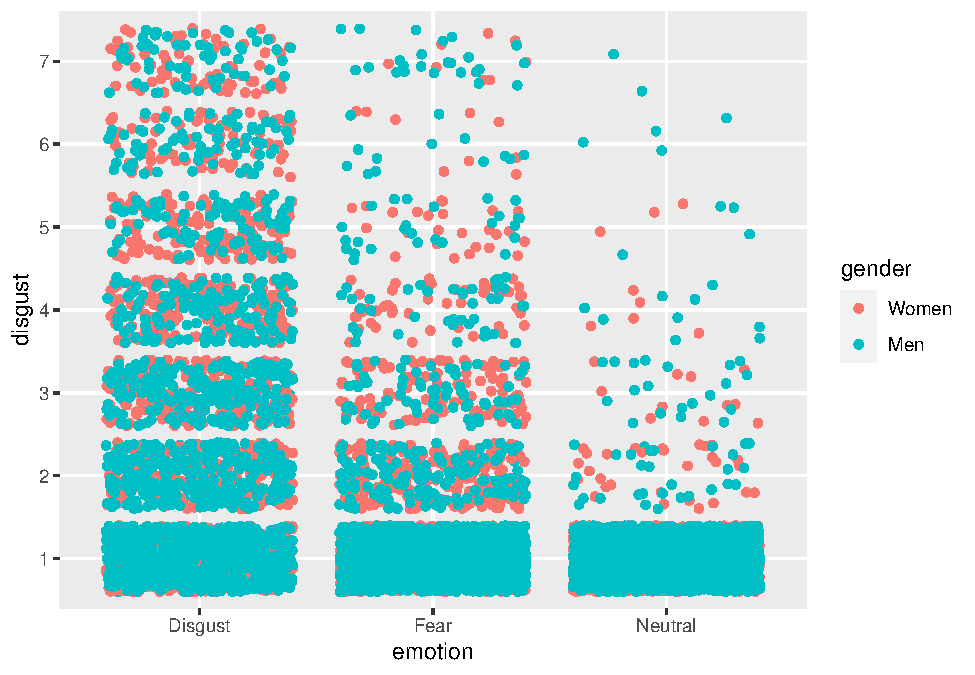
\includegraphics{Dap_pro2_files/figure-latex/unnamed-chunk-2-1.pdf}

\begin{Shaded}
\begin{Highlighting}[]
\NormalTok{a}\OtherTok{=}\DecValTok{9349}
\NormalTok{Item }\OtherTok{\textless{}{-}} \FunctionTok{rev}\NormalTok{(}\FunctionTok{sort}\NormalTok{(}\FunctionTok{unique}\NormalTok{(Data}\SpecialCharTok{$}\NormalTok{emotion)))}
\NormalTok{one }\OtherTok{\textless{}{-}}\NormalTok{ (}\DecValTok{6611}\SpecialCharTok{/}\NormalTok{a)}\SpecialCharTok{*}\DecValTok{100}
\NormalTok{two }\OtherTok{\textless{}{-}}\NormalTok{ (}\DecValTok{972}\SpecialCharTok{/}\NormalTok{a)}\SpecialCharTok{*}\DecValTok{100}
\NormalTok{three }\OtherTok{\textless{}{-}}\NormalTok{ (}\DecValTok{706}\SpecialCharTok{/}\NormalTok{a)}\SpecialCharTok{*}\DecValTok{100}
\NormalTok{four }\OtherTok{\textless{}{-}}\NormalTok{ (}\DecValTok{432}\SpecialCharTok{/}\NormalTok{a)}\SpecialCharTok{*}\DecValTok{100}
\NormalTok{five }\OtherTok{\textless{}{-}}\NormalTok{ (}\DecValTok{288}\SpecialCharTok{/}\NormalTok{a)}\SpecialCharTok{*}\DecValTok{100}
\NormalTok{six }\OtherTok{\textless{}{-}}\NormalTok{ (}\DecValTok{174}\SpecialCharTok{/}\NormalTok{a)}\SpecialCharTok{*}\DecValTok{100}
\NormalTok{seven }\OtherTok{\textless{}{-}}\NormalTok{ (}\DecValTok{166}\SpecialCharTok{/}\NormalTok{a)}\SpecialCharTok{*}\DecValTok{100}
\NormalTok{df }\OtherTok{\textless{}{-}} \FunctionTok{data.frame}\NormalTok{(Item, one, two, three, four, five, six, seven)}
\DocumentationTok{\#\# Rename Cols}
\NormalTok{df }\OtherTok{\textless{}{-}}\NormalTok{ df }\SpecialCharTok{\%\textgreater{}\%}
\FunctionTok{rename}\NormalTok{(}\StringTok{"1 (low)"} \OtherTok{=}\NormalTok{ one, }\StringTok{"2"} \OtherTok{=}\NormalTok{ two, }\StringTok{"3"} \OtherTok{=}\NormalTok{ three, }\StringTok{"4"} \OtherTok{=}\NormalTok{ four, }\StringTok{"5"} \OtherTok{=}\NormalTok{ five, }\StringTok{"6"}\OtherTok{=}\NormalTok{ six, }\StringTok{"7 (high)"}\OtherTok{=}\NormalTok{ seven)}
\FunctionTok{summary}\NormalTok{(df)}
\end{Highlighting}
\end{Shaded}

\begin{verbatim}
##       Item      1 (low)            2              3               4        
##  Disgust:1   Min.   :70.71   Min.   :10.4   Min.   :7.552   Min.   :4.621  
##  Fear   :1   1st Qu.:70.71   1st Qu.:10.4   1st Qu.:7.552   1st Qu.:4.621  
##  Neutral:1   Median :70.71   Median :10.4   Median :7.552   Median :4.621  
##              Mean   :70.71   Mean   :10.4   Mean   :7.552   Mean   :4.621  
##              3rd Qu.:70.71   3rd Qu.:10.4   3rd Qu.:7.552   3rd Qu.:4.621  
##              Max.   :70.71   Max.   :10.4   Max.   :7.552   Max.   :4.621  
##        5               6            7 (high)    
##  Min.   :3.081   Min.   :1.861   Min.   :1.776  
##  1st Qu.:3.081   1st Qu.:1.861   1st Qu.:1.776  
##  Median :3.081   Median :1.861   Median :1.776  
##  Mean   :3.081   Mean   :1.861   Mean   :1.776  
##  3rd Qu.:3.081   3rd Qu.:1.861   3rd Qu.:1.776  
##  Max.   :3.081   Max.   :1.861   Max.   :1.776
\end{verbatim}

\begin{Shaded}
\begin{Highlighting}[]
\DocumentationTok{\#\# Pretty Plot}
\CommentTok{\# plot(likert(summary = df))}
\CommentTok{\# + guides(fill = guide\_legend(name="Subjective evaluation"))}
\CommentTok{\# + labs(title = "Subjective evaluation of disgust across all pairs of words")}
\CommentTok{\# + labs(y = "Percentage of Likert answers")}
\CommentTok{\# + labs(x="Word pairs\textquotesingle{} emotions")}
\CommentTok{\# + theme(plot.title = element\_text(hjust = 0.5))}
\CommentTok{\# + theme(plot.title = element\_text(size = rel(1.5)))}
\CommentTok{\# + theme( legend.box.background = element\_rect(), legend.box.margin = margin(6, 6, 6, 6), legend.position = "top")}
\end{Highlighting}
\end{Shaded}

\hypertarget{modelisation}{%
\section{Modelisation}\label{modelisation}}

\begin{Shaded}
\begin{Highlighting}[]
\NormalTok{disgust2}\OtherTok{\textless{}{-}}\FunctionTok{as.numeric}\NormalTok{(disgust)}
\NormalTok{m1}\FloatTok{.0} \OtherTok{=} \FunctionTok{lm}\NormalTok{(disgust2}\SpecialCharTok{\textasciitilde{}}\NormalTok{emotion}\SpecialCharTok{*}\NormalTok{gender, }\AttributeTok{data=}\NormalTok{Data)}
\FunctionTok{plot}\NormalTok{(m1}\FloatTok{.0}\NormalTok{)}
\end{Highlighting}
\end{Shaded}

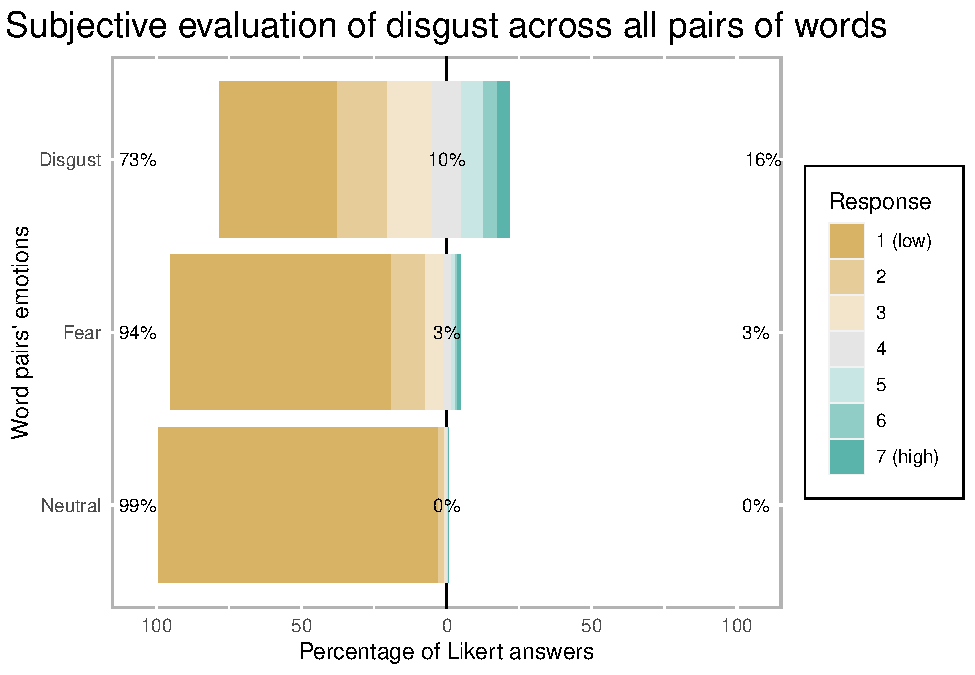
\includegraphics{Dap_pro2_files/figure-latex/unnamed-chunk-4-1.pdf}
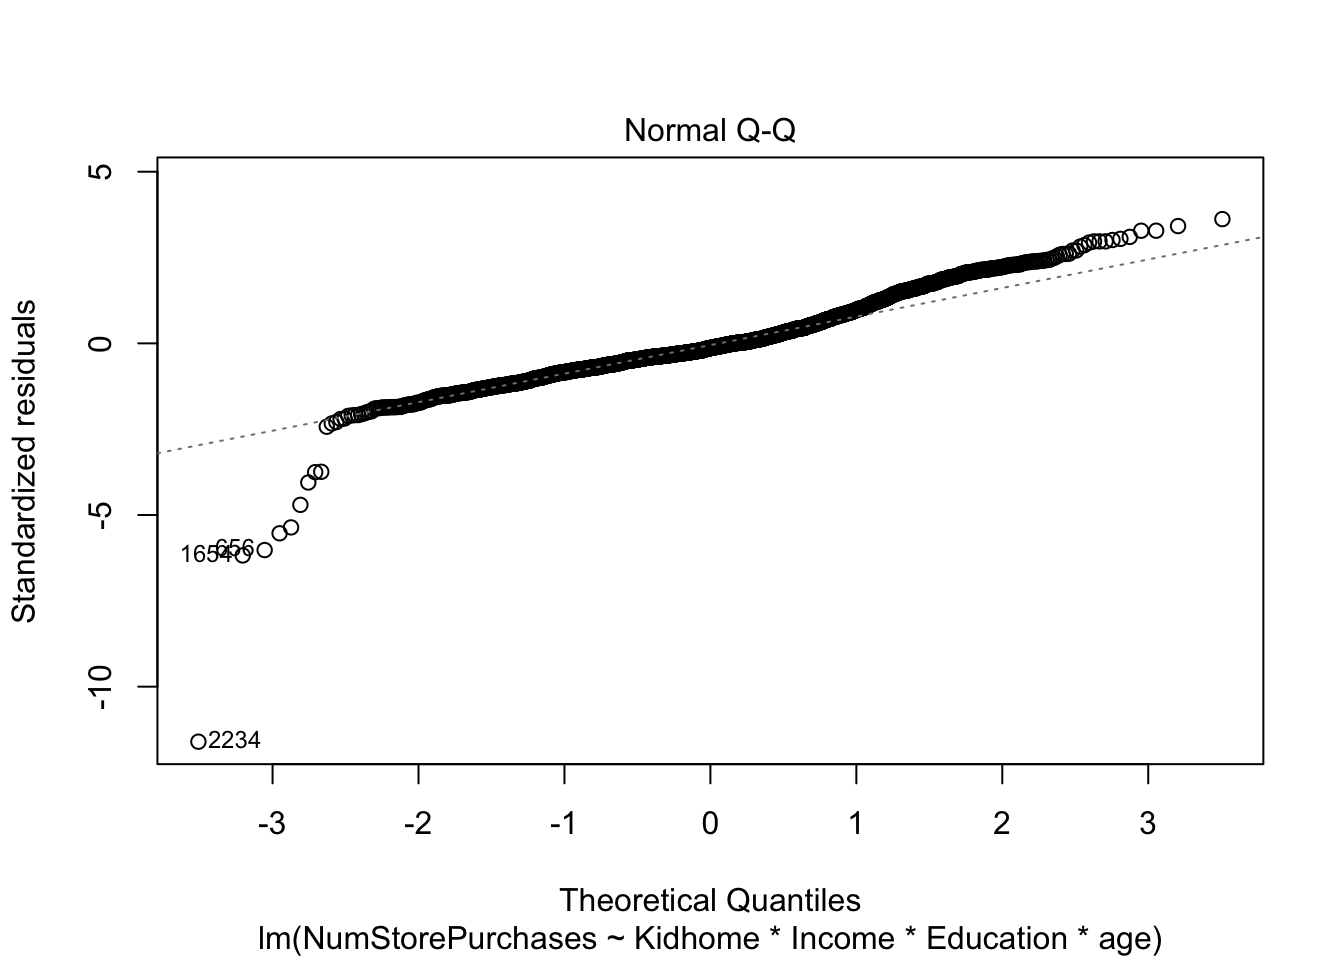
\includegraphics{Dap_pro2_files/figure-latex/unnamed-chunk-4-2.pdf}
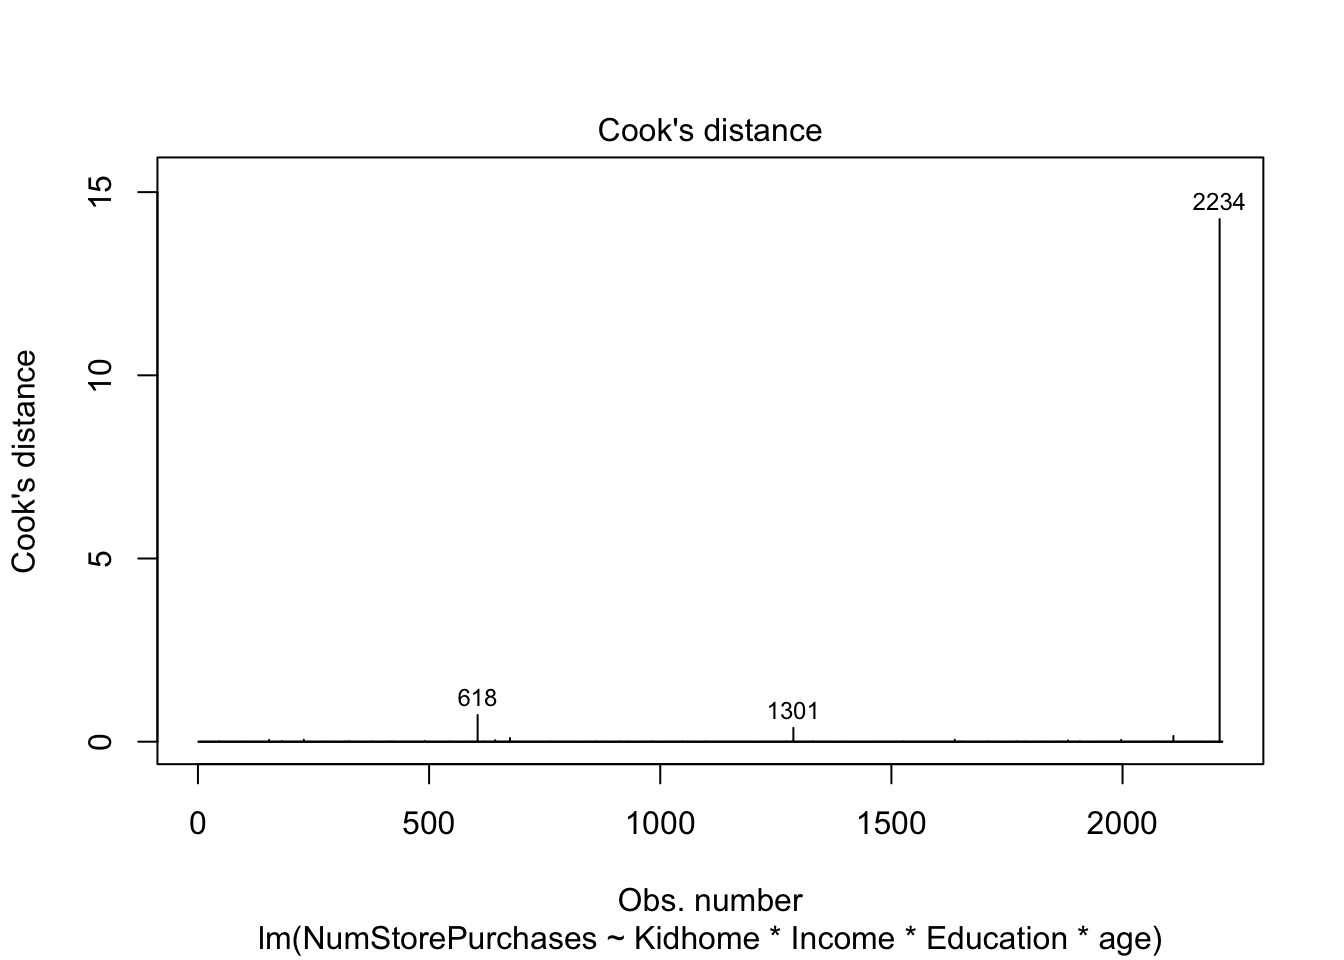
\includegraphics{Dap_pro2_files/figure-latex/unnamed-chunk-4-3.pdf}
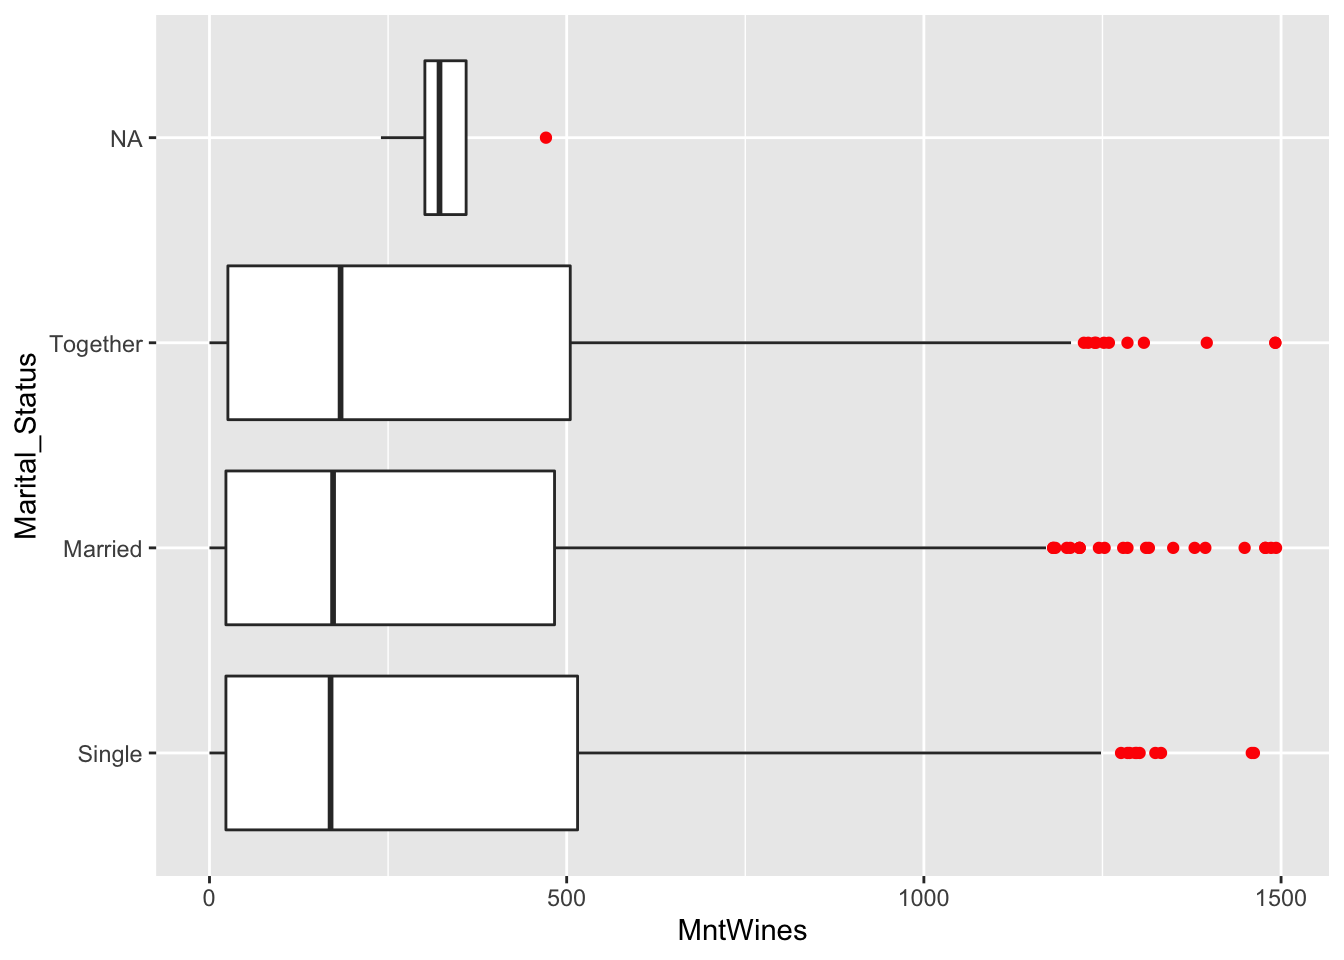
\includegraphics{Dap_pro2_files/figure-latex/unnamed-chunk-4-4.pdf}

\begin{Shaded}
\begin{Highlighting}[]
\NormalTok{sjPlot}\SpecialCharTok{::}\FunctionTok{plot\_model}\NormalTok{(m1}\FloatTok{.0}\NormalTok{,}\AttributeTok{type =} \StringTok{"diag"}\NormalTok{)[[}\DecValTok{3}\NormalTok{]]}
\end{Highlighting}
\end{Shaded}

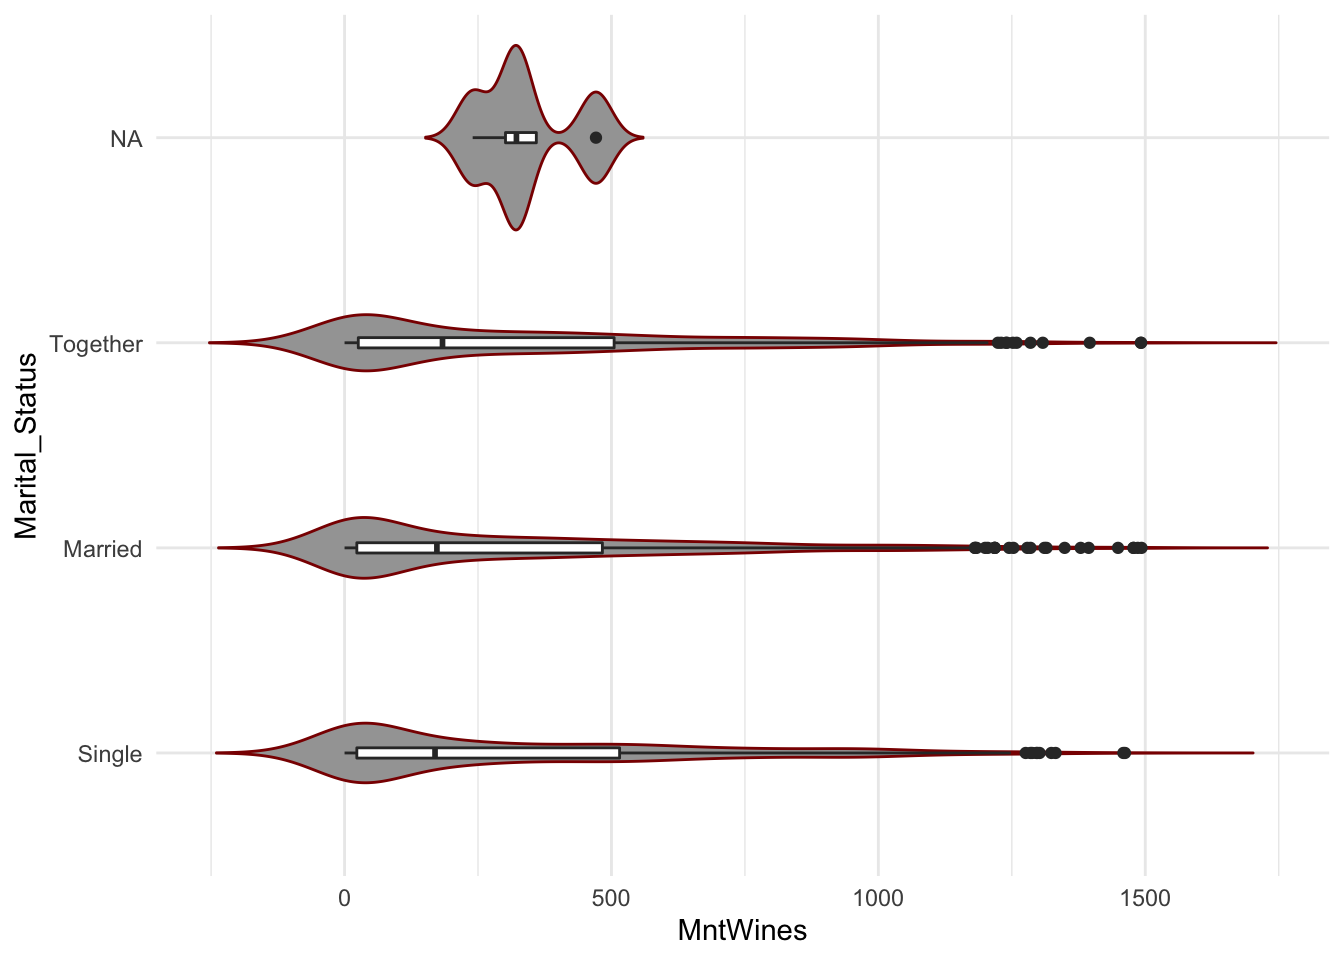
\includegraphics{Dap_pro2_files/figure-latex/unnamed-chunk-4-5.pdf}

\begin{Shaded}
\begin{Highlighting}[]
\CommentTok{\#best method}

\NormalTok{m1}\FloatTok{.2} \OtherTok{=} \FunctionTok{clm}\NormalTok{(disgust }\SpecialCharTok{\textasciitilde{}}\NormalTok{ emotion }\SpecialCharTok{*}\NormalTok{ gender, }\AttributeTok{data =}\NormalTok{ Data)}
\NormalTok{m2}\FloatTok{.2} \OtherTok{=} \FunctionTok{clmm}\NormalTok{(disgust }\SpecialCharTok{\textasciitilde{}}\NormalTok{ emotion }\SpecialCharTok{*}\NormalTok{ gender }\SpecialCharTok{+}\NormalTok{ (}\DecValTok{1}\SpecialCharTok{|}\NormalTok{subjects), }\AttributeTok{data =}\NormalTok{ Data)}
\NormalTok{m3}\FloatTok{.2} \OtherTok{=} \FunctionTok{clmm}\NormalTok{(disgust }\SpecialCharTok{\textasciitilde{}}\NormalTok{ emotion }\SpecialCharTok{*}\NormalTok{ gender }\SpecialCharTok{+}\NormalTok{ (emotion }\SpecialCharTok{|}\NormalTok{ subjects), }\AttributeTok{data =}\NormalTok{ Data)}
\FunctionTok{extractAIC}\NormalTok{(m1}\FloatTok{.2}\NormalTok{)}
\end{Highlighting}
\end{Shaded}

\begin{verbatim}
## [1]    11.00 17242.03
\end{verbatim}

\begin{Shaded}
\begin{Highlighting}[]
\FunctionTok{extractAIC}\NormalTok{(m2}\FloatTok{.2}\NormalTok{)}
\end{Highlighting}
\end{Shaded}

\begin{verbatim}
## [1]    12.00 16204.65
\end{verbatim}

\begin{Shaded}
\begin{Highlighting}[]
\FunctionTok{extractAIC}\NormalTok{(m3}\FloatTok{.2}\NormalTok{)}
\end{Highlighting}
\end{Shaded}

\begin{verbatim}
## [1]    17.00 16075.78
\end{verbatim}

\begin{Shaded}
\begin{Highlighting}[]
\CommentTok{\# {-}{-}\textgreater{} m3.2}
\end{Highlighting}
\end{Shaded}

\begin{Shaded}
\begin{Highlighting}[]
\CommentTok{\#best model}
\NormalTok{m3}\FloatTok{.2} \OtherTok{=} \FunctionTok{clmm}\NormalTok{(disgust }\SpecialCharTok{\textasciitilde{}}\NormalTok{ emotion }\SpecialCharTok{*}\NormalTok{ gender }\SpecialCharTok{+}\NormalTok{ (emotion }\SpecialCharTok{|}\NormalTok{ subjects), }\AttributeTok{data =}\NormalTok{ Data)}
\NormalTok{m3}\FloatTok{.1} \OtherTok{=} \FunctionTok{clmm}\NormalTok{(disgust }\SpecialCharTok{\textasciitilde{}}\NormalTok{ emotion }\SpecialCharTok{+}\NormalTok{ gender }\SpecialCharTok{+}\NormalTok{ (emotion }\SpecialCharTok{|}\NormalTok{ subjects), }\AttributeTok{data =}\NormalTok{ Data)}
\NormalTok{m3}\FloatTok{.0} \OtherTok{=} \FunctionTok{clmm}\NormalTok{(disgust }\SpecialCharTok{\textasciitilde{}}\NormalTok{ emotion }\SpecialCharTok{+}\NormalTok{ (emotion }\SpecialCharTok{|}\NormalTok{ subjects), }\AttributeTok{data =}\NormalTok{ Data)}

\FunctionTok{extractAIC}\NormalTok{(m3}\FloatTok{.2}\NormalTok{)}
\end{Highlighting}
\end{Shaded}

\begin{verbatim}
## [1]    17.00 16075.78
\end{verbatim}

\begin{Shaded}
\begin{Highlighting}[]
\FunctionTok{extractAIC}\NormalTok{(m3}\FloatTok{.1}\NormalTok{)}
\end{Highlighting}
\end{Shaded}

\begin{verbatim}
## [1]    15.00 16076.82
\end{verbatim}

\begin{Shaded}
\begin{Highlighting}[]
\FunctionTok{extractAIC}\NormalTok{(m3}\FloatTok{.0}\NormalTok{)}
\end{Highlighting}
\end{Shaded}

\begin{verbatim}
## [1]    14.00 16074.89
\end{verbatim}

\begin{Shaded}
\begin{Highlighting}[]
\CommentTok{\#{-}{-}\textgreater{} m3.0}
\end{Highlighting}
\end{Shaded}

\begin{Shaded}
\begin{Highlighting}[]
\FunctionTok{summary}\NormalTok{(m3}\FloatTok{.0}\NormalTok{)}
\end{Highlighting}
\end{Shaded}

\begin{verbatim}
## Cumulative Link Mixed Model fitted with the Laplace approximation
## 
## formula: disgust ~ emotion + (emotion | subjects)
## data:    Data
## 
##  link  threshold nobs logLik   AIC      niter       max.grad cond.H 
##  logit flexible  9349 -8023.44 16074.89 2338(11710) 8.96e-03 4.9e+02
## 
## Random effects:
##  Groups   Name           Variance Std.Dev. Corr          
##  subjects (Intercept)    0.9960   0.9980                 
##           emotionFear    0.6444   0.8027   -0.050        
##           emotionNeutral 0.3974   0.6304   -0.699  0.404 
## Number of groups:  subjects 52 
## 
## Coefficients:
##                Estimate Std. Error z value Pr(>|z|)    
## emotionFear     -2.0596     0.1314  -15.68   <2e-16 ***
## emotionNeutral  -3.9909     0.1497  -26.66   <2e-16 ***
## ---
## Signif. codes:  0 '***' 0.001 '**' 0.01 '*' 0.05 '.' 0.1 ' ' 1
## 
## Threshold coefficients:
##     Estimate Std. Error z value
## 1|2  -0.5346     0.1437  -3.721
## 2|3   0.3387     0.1435   2.359
## 3|4   1.1585     0.1445   8.018
## 4|5   1.8831     0.1467  12.834
## 5|6   2.6467     0.1515  17.466
## 6|7   3.4641     0.1619  21.403
\end{verbatim}

\begin{Shaded}
\begin{Highlighting}[]
\NormalTok{RVAideMemoire}\SpecialCharTok{::}\FunctionTok{Anova.clmm}\NormalTok{(m3}\FloatTok{.0}\NormalTok{, }\AttributeTok{type =} \StringTok{"II"}\NormalTok{) }\CommentTok{\#or type = "III" depending on the context}
\end{Highlighting}
\end{Shaded}

\begin{verbatim}
## Analysis of Deviance Table (Type II tests)
## 
## Response: disgust
##         LR Chisq Df Pr(>Chisq)    
## emotion    153.6  2  < 2.2e-16 ***
## ---
## Signif. codes:  0 '***' 0.001 '**' 0.01 '*' 0.05 '.' 0.1 ' ' 1
\end{verbatim}

\hypertarget{diagnostic-of-the-model}{%
\section{Diagnostic of the model}\label{diagnostic-of-the-model}}

\begin{Shaded}
\begin{Highlighting}[]
\CommentTok{\#plot(m3.0) \#do not work}
\CommentTok{\#autoplot.resid(m3.0) \#\#do not work}
\CommentTok{\#read this : David W.. Hosmer, Lemeshow, S., \& Rodney X.. Sturdivant. (2000). Applied logistic regression. New York: Wiley. {-}{-}\textgreater{} §5}

\NormalTok{sjPlot}\SpecialCharTok{::}\FunctionTok{tab\_model}\NormalTok{(m3}\FloatTok{.0}\NormalTok{)}
\end{Highlighting}
\end{Shaded}

~

disgust

Predictors

Odds Ratios

CI

p

1\textbar2

0.59

0.44~--~0.78

\textless0.001

2\textbar3

1.40

1.06~--~1.86

0.018

3\textbar4

3.19

2.40~--~4.23

\textless0.001

4\textbar5

6.57

4.93~--~8.76

\textless0.001

5\textbar6

14.11

10.48~--~18.99

\textless0.001

6\textbar7

31.95

23.26~--~43.88

\textless0.001

emotion {[}Fear{]}

0.13

0.10~--~0.16

\textless0.001

emotion {[}Neutral{]}

0.02

0.01~--~0.02

\textless0.001

Random Effects

σ2

3.29

τ00 subjects

1.00

τ11 subjects.emotionFear

0.64

τ11 subjects.emotionNeutral

0.40

ρ01

-0.05

-0.70

ICC

0.24

N subjects

52

Observations

9349

Marginal R2 / Conditional R2

0.381 / 0.528

\begin{Shaded}
\begin{Highlighting}[]
\FunctionTok{autoplot.clm}\NormalTok{(m1}\FloatTok{.2}\NormalTok{, }\AttributeTok{what=}\StringTok{"qq"}\NormalTok{)}
\end{Highlighting}
\end{Shaded}

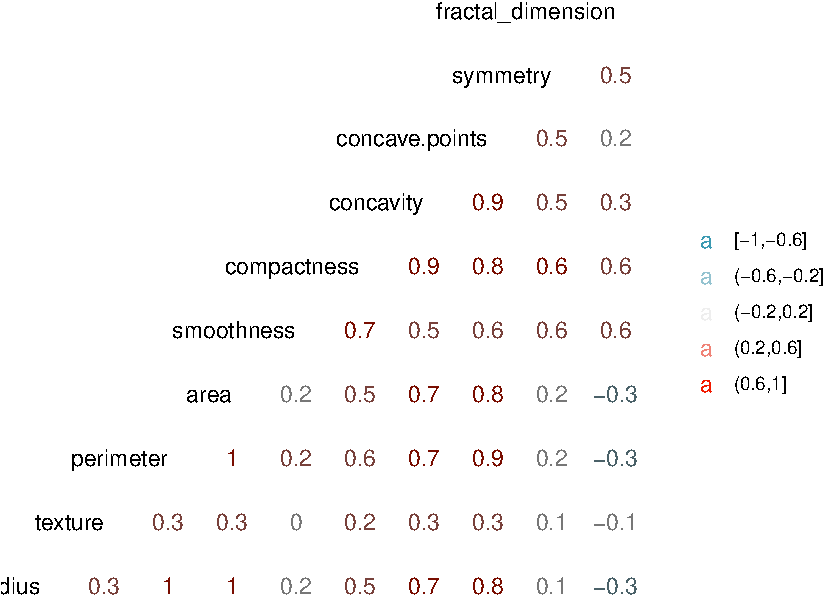
\includegraphics{Dap_pro2_files/figure-latex/unnamed-chunk-7-1.pdf}

\begin{Shaded}
\begin{Highlighting}[]
\FunctionTok{plot}\NormalTok{(m1}\FloatTok{.0}\NormalTok{, }\AttributeTok{which =} \DecValTok{2}\NormalTok{)}
\end{Highlighting}
\end{Shaded}

\includegraphics{Dap_pro2_files/figure-latex/unnamed-chunk-7-2.pdf}

\end{document}
